\newpage
\section{Лекция 13}
\subsection{Итеративное решение систем линейных уравнений.}
$$Ax=b~~(1)$$
Если матрица $A$ не является симметричной (и положительно определенной), то надо перейти от (1) к нормальной системе $$A^*Ax=A^*b$$
\\
\textbf{Метод Крылова.}\\
Для любого оператора существует минимальный многочлен $\varphi(x)$
$$\varphi(x)=x^m+p_{m-1}x^{m-1}+\cdots+p_1x+p_0$$
\textbf{Задача:} найти коэффициенты $\varphi(x)$
$$(A^m+p_{m-1}A^{m-1}+\cdots+p_1A+p_0E)v=0$$
$L=<v_0, Av_0,\cdots,A^{m-1}v_0>$ --- зависит от $v_0$, причем $v_{m-1}=Av_{m-2}$.\\
Выразим:
$$A^mv=-p_{m-1}A^{m-1}v-\cdots-p_0Ev~~(2)$$
Замечание: $L(v_0)$ инвариантно относительно линейного оператора $A$.\\
\textbf{Метод:} возьмем $v_0$ и решим (2) относительно $m$ неизвестных $p_0,\cdots,p_{m-1}$.\\
\\
Характеристический многочлен $$\chi_A(\lambda)=det(A-\lambda E)$$
Если матрица приводится к виду
\[ 
J=
\left(
\begin{BMAT}[8pt]{ccc:ccc}{ccc:ccc}
\lambda_1 & 1  & 0 & &  &  \\
\vdots & \ddots & 1 &  & 0  & \\
0 & \cdots & \lambda_1 &  & & \\
&  & & \lambda_2 & 1 & 0  \\
& 0 &  & \vdots & \ddots & 1  \\
&  &  & 0 & \cdots & \lambda_2   \\
\end{BMAT} 
\right)
\]
где кратность $\lambda_1$ равна $k$, а кратность $\lambda_2$ равна $m$, то
$$\chi_J(\lambda)=(\lambda_1-\lambda)^k(\lambda_2-\lambda)^m$$
\begin{definition}
    \textbf{Циклическая клетка} --- это матрица вида
\[C_n=\begin{pmatrix}
0 & 0 & \cdots & 0 & a_0 \\
1 & 0 & \cdots & 0 & a_1 \\
0 & 1 & \cdots & 0 & a_2 \\
\vdots & \vdots & \ddots & \vdots & \vdots \\
0 & 0 & \cdots & 1 & a_{n-1} \\
\end{pmatrix}\]
\end{definition}
Найдем характеристический многочлен у циклической клетки.\\
\[C_2=\begin{pmatrix}
0 & a_0 \\
1 & a_1 \\
\end{pmatrix}\]
\[\chi_{C_2}= det(C_2-\lambda E)=\begin{vmatrix}
-\lambda & a_0 \\
1 & a_1-\lambda \\
\end{vmatrix}=\lambda^2-a_1\lambda-a_0\]
\[C_3=\begin{pmatrix}
0 & 0 & a_0 \\
1 &  0 & a_1 \\
0 & 1 & a_2 \\
\end{pmatrix}\]
\[\chi_{C_3}= det(C_3-\lambda E)=\begin{vmatrix}
-\lambda & 0 & a_0 \\
1 & -\lambda & a_1\\
0 & 1 & a_2-\lambda \\
\end{vmatrix}=-\lambda^3+\lambda^2a_2+\lambda a_1+a_0\]
Тогда для $C_n$ получим
$$\chi_{C_n}=det(C_n-\lambda E)=(-1)^n(\lambda^n-a_{n-1}\lambda^{n-1}-\cdots-a_0)$$
\\
Однако не все матрицы можно привести к такому виду.
\begin{definition}
    \textbf{Фробениусова форма} --- это матрица вида
\[F_n=\begin{pmatrix}
a_{n-1} & a_{n-2} & \cdots & a_1 & a_0 \\
1 & 0 & \cdots & 0 & 0 \\
0 & 1 & \cdots & 0 & 0 \\
\vdots & \vdots & \ddots & \vdots & \vdots \\
0 & 0 & \cdots & 1 & 0 \\
\end{pmatrix}\]
Данная матрица получена отражением относительно побочной диагонали.
\end{definition}
Как приводить матрицу к фробениусовой форме?\\
Надо составить базис. Выбрем $v_0$ случайным образом.\\
$$v_0, Av_0=v_1, Av_1=v_2, Av_2=v_3,\cdots$$
Эти векторы $v_0, v_1,\cdots$ --- базис линейного пространства.\\
$$v_{n-1}=A^{n-1}v_0,~v_n=A^{n-1}v_1=a_0v_0+a_1v_1+\cdots +a_{n-1}v_{n-1}$$
\[(v_0)_v=\begin{pmatrix}
1 \\
0 \\
\vdots \\
0
\end{pmatrix},~(v_1)_v=(Av_0)_v=\begin{pmatrix}
0 \\
1 \\
\vdots \\
0
\end{pmatrix}=0\cdot v_0+1\cdot v_1+0\cdot v_2+\cdots\]
\[A_v=((Av_0)_v~|~(Av_1)_v~|~\cdots)=\begin{pmatrix}
0 & 0 & \cdots & 0 & a_0 \\
1 & 0 & \cdots & 0 & a_1 \\
0 & 1 & \cdots & 0 & a_2 \\
\vdots & \vdots & \ddots & \vdots & \vdots \\
0 & 0 & \cdots & 1 & a_{n-1} \\
\end{pmatrix}\]
$$A_1=A\cdot M_{n-1}$$
\[A=\begin{pmatrix}
a_{11} & \cdots & a_{1, n-1} & a_{1n} \\
\cdots & \cdots & \cdots & \cdots \\
a_{n1} & \cdots & a_{n, n-1} & a_{nn} \\
\end{pmatrix}\]
\[ 
M_{n-1}=
\left(
\begin{BMAT}[8pt]{ccc:cc}{ccc:cc}
1 & \cdots  & 0 & 0 & 0   \\
\vdots & \ddots & \vdots & \vdots & \vdots   \\
0 & \cdots & 1 & 0 & 0 \\
-\cfrac{a_{n1}}{a_{n, n-1}}& \cdots & \cdots & \cfrac{1}{a_{n, n-1}} & -\cfrac{a_{nn}}{a_{n, n-1}}  \\
0 & \cdots & 0 & 0 & 1  \\
\end{BMAT} 
\right)
\]
\[ 
A_1=AM_{n-1}=
\left(
\begin{BMAT}[8pt]{ccccc}{c:c}
&        & *  &    &  \\
0 & \cdots & 0 & 1  & 0 \\
\end{BMAT} 
\right)
\]
\[ 
B_1=M_{n-1}^{-1}AM_{n-1}=
\left(
\begin{BMAT}[8pt]{ccccc}{c:c}
&        & *  &    &  \\
0 & \cdots & 0 & 1  & 0 \\
\end{BMAT} 
\right)
\]
\[ 
M_{n-1}^{-1}=
\left(
\begin{BMAT}[8pt]{ccc:c}{ccc:cc}
1 & \cdots  & 0 & 0    \\
\vdots & \ddots & \vdots & \vdots    \\
0 & \cdots & 1 & 0  \\
a_{n1}& \cdots & a_{n, n-1} & a_{nn}  \\
0 & \cdots & 0 &  1  \\
\end{BMAT} 
\right)
\]
\textbf{Интерполяционный метод.}\\
$\chi_A(\lambda)$ --- многочлен степени $m$ --- вычисляется как интерполяционный многочлен Лагранжа по значениям в $(m+1)$ точке.\\
\\
Характеристический многочлен $$\chi_A(\lambda)=det(A-\lambda E),~~\lambda=0,1,\cdots,m$$
То есть, надо $m$ раз вычислить определитель.
\subsection{Метод итераций}
$$\bar x=P\bar x+\bar b$$
Итеративный шаг: $x^{k+1}=Px^k+\bar b$.\\
\\
Матрица называется симметрической, если $A^T=A,~A$ --- действительная.\\
$A^*A$ --- симметрическая матрица.\\
\\
Пусть $A^*=A$ --- эрмитова матрица (например, симметическая). Нам неизвестны $\lambda_1,\cdots,\lambda_n$ --- собственные значения и соответствующие им собственные векторы $X_1,\cdots, X_n$.\\
Пусть 
\[X_1=\begin{pmatrix}
x_1^1\\
x_2^1\\
\vdots\\
x_n^1
\end{pmatrix}\]
Если $X_1$ --- собственный вектор, то и $c\cdot X$ --- собственный вектор, то есть $X_1$ определен с точностью до пропорциональности. Считаем $x_n^1=1$.\\
Получим $A\bar x_1=\lambda_1 \bar x_1$ или
\\ \\
$
\left\{
\begin{array}{lcl}
a_{11}x_1^1+\cdots +a_{1n}\cdot 1 =\lambda_1 x_1^1\\
\cdots\\
a_{n-1, 1}x_1^1+\cdots +a_{n-1, n}\cdot 1=\lambda_1 x_{n-1}^1\\
a_{n1}x_1^1+\cdots +a_{nn}\cdot 1 =\lambda_1\\
\end{array}
\right.
$
\\ 
\\
$
\left\{
\begin{array}{lcl}
\lambda_1= a_{n1}x_1^1+\cdots +a_{nn}\\
x_1^1=\cfrac{1}{\lambda_1}(a_{11}x_1^1+\cdots +a_{1n})\\
\cdots\\
x_{n-1}^1=\cfrac{1}{\lambda_1}(a_{n-1, 1}x_1^1+\cdots +a_{n-1, n})\\
\end{array}
\right.
$
\\
$$\bar Y=f(\bar Y)$$
Итеративный процесс
\\ \\
$
\left\{
\begin{array}{lcl}
\lambda_1^{(k+1)}= a_{n1}x_1^{1(k)}+\cdots +a_{nn}\\
x_1^{1(k+1)}=\cfrac{1}{\lambda_1^{(k)}}(a_{11}x_1^{1(k)}+\cdots +a_{1n})\\
\cdots\\
x_{n-1}^{1(k+1)}=\cfrac{1}{\lambda_1^{(k)}}(a_{n-1, 1}x_1^{1(k)}+\cdots +a_{n-1, n})\\
\end{array}
\right.
$
\\ \\
Начальное условие $\lambda_1^0=a_{nn}$, $x_1^0=\cfrac{a_{1n}}{a_{nn}}, \cdots$.\\
\\
Для $X_2$ те же уравнения (аналогичные) и условие $<X_1, X_2>=0$.
$$x_1^1x_1^2+\cdots+x_n^1x_n^2=0$$
\\
\textbf{Приведение к виду, удобному для итераций.}\\
Приведем систему уравнений $A\bar x=\bar b$ к виду $A^*Ax=A^*b$.\\
Для итеративного метода
$$\bar x=P \bar x+\bar B$$
$$x=(E-A)x+b$$
Возьмем число $\tau:$ $\tau Ax=\tau b$\\
$$x=(E-\tau A)x+\tau b,~~P=E-\tau A$$
Собственные значения матрицы $P:$ $\lambda_i(P)=1-\tau \lambda_i (A)$.\\
\[\begin{pmatrix}
\lambda_1(P) & \cdots & 0\\
\vdots & \ddots & \vdots\\
0 & \cdots & \lambda_n(P)\\
\end{pmatrix}=\begin{pmatrix}
1 & \cdots & 0\\
\vdots & \ddots & \vdots\\
0 & \cdots & 1\\
\end{pmatrix}- \tau \begin{pmatrix}
\lambda_1(A) & \cdots & 0\\
\vdots & \ddots & \vdots\\
0 & \cdots & \lambda_n(A)\\
\end{pmatrix}\]
Пусть $m\leqslant |\lambda_i(A)|\leqslant M$, то есть $M=\varsigma(A)=\rho(A),~m=\cfrac{1}{\varsigma(A^{-1})}=\cfrac{1}{\rho(A^{-1})}$.\\
Это верно только для $\lambda_i \geqslant 0$.\\
$$\underset{i}{max}|\lambda_i(P)| \to min$$
$$\underset{i}{max}|\lambda_i(P)| \leqslant max\{|1-\tau m|, |1-\tau M|\}$$
Какое выбрать $\tau$?
\begin{center}
    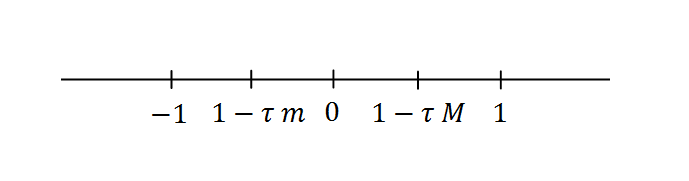
\includegraphics[scale=0.8]{l13_1.png}\end{center}
Лучше взять $\tau<\cfrac{2}{m+M}$, чем $\tau>\cfrac{2}{m+M}$. Лучше всего выбрать $\tau=\cfrac{2}{m+M}$.\\ \\
Если $\tau=\tau_0=\cfrac{2}{m+M}$, то $\rho(P)=max\{|1-\tau_0 m|, |1-\tau_0 M|\}=max \bigg\{ \left |\cfrac{M-m}{m+M} \right |, \left |\cfrac{m-M}{m+M} \right| \bigg\}=\cfrac{M-m}{M+m}=\cfrac{\chi_2-1}{\chi_2+1}$, где $\chi_2(A)=\cfrac{M}{m}$ --- число обусловленности.\\
\\
Если нет собственных значений, то можно взять $\tau=\cfrac{2}{a}$, где $a \geqslant ||A|| \geqslant \rho(A)$ (какая-то норма $||A||=||A||_{\infty }$ или $||A||=\cfrac{1}{n}\sum\limits_{i, j} |a_{ij}|$).\\
\\
\textbf{Пример 1.}\\
Методом итераций найти собственные значения.
\[A=\begin{pmatrix}
6 & -2 & 2\\
-2 & 5 & 0\\
2 & 0 & 7\\
\end{pmatrix}\]
Умножим на 
\[\bar x_1=\begin{pmatrix}
x_1\\
x_2\\
1\\
\end{pmatrix}\]
(предполагаем, что найдется такой вектор).
$$A\bar x_1=\lambda \bar x_1$$
$
\left\{
\begin{array}{lcl}
6x_1-2x_2+2=\lambda x_1\\
-2x_1+5x_2=\lambda x_2\\
2x_1+7=\lambda x_3=\lambda\\
\end{array}
\right.
$
\\
\\
$
\left\{
\begin{array}{lcl}
\lambda^{(k+1)}=2x_1^{(k)}+7\\
x_1^{(k+1)}=\cfrac{1}{\lambda^{(k)}}(6x_1^{(k)}-2x_2^{(k)}+2)\\
x_2^{(k+1)}=\cfrac{1}{\lambda^{(k)}}=\cfrac{1}{\lambda^{(k)}}(-2x_1^{(k)}+5x_2^{(k)})\\
\end{array}
\right.
$
\\
\\
Через итерации получим 
\[\lambda_1=9,~v_1=\begin{pmatrix}
1\\
-\cfrac{1}{2}\\
1\\
\end{pmatrix}\]
Найдем $\lambda_2, v_2$.\\
Для $\bar x_2$ те же уравнения и $<\bar x_1, \bar x_2>=0$, то есть \\
\\
$
\left\{
\begin{array}{lcl}
6x_1-2x_2+2x_3=\lambda x_1\\
-2x_1+5x_2=\lambda x_2\\
2x_1+7x_3=\lambda x_3\\
x_1-\cfrac{1}{2}x_2+x_3=0\\
\end{array}
\right.
$
\\
\\
Так как сумма собственный значений равна следу = 18, то из этого выражения, зная $\lambda_1, \lambda_2$ можно найти $\lambda_3$.
\subsection{Домашнее задание 13}\begin{enumerate}
    \item Дорешать Пример 1 с лекции.
    \item Методом Крылова найти минимальный характеристический многочлен.
    \begin{enumerate}
        \item \[A = \begin{pmatrix}[r]
        -1 & 0 & 1 & 2\\
        7 & 1 & 0 & 1\\
        -1 & 1 & 8 & 11\\
        0 & 0 & 1 & 0\\
        \end{pmatrix}\]
        \item \[A = \begin{pmatrix}[r]
        1 & -3 & -1\\
        -3 & 1 & 1\\
        -1 & 1 & 5\\
        \end{pmatrix}\]
    \end{enumerate}
    \item Методом Данилевского найти характеристический многочлен.
    \[A = \begin{pmatrix}[r]
    3 & 1 & 2 & 4\\
    7 & 1 & 0 & 1\\
    2 & 1 & 2 & 3\\
    4 & 1 & 2 & 2\\
    \end{pmatrix}\]
    \item Найти собственные значения и собственные векторы методом итераций.
    \[A = \begin{pmatrix}[r]
    18 & 6 & -6\\
    6 & 21 & 0\\
    -6 & 0 & 16\\
    \end{pmatrix}\]
\end{enumerate}